\documentclass[11pt,a4paper,]{article}
\usepackage{lmodern}

\usepackage{amssymb,amsmath}
\usepackage{ifxetex,ifluatex}
\usepackage{fixltx2e} % provides \textsubscript
\ifnum 0\ifxetex 1\fi\ifluatex 1\fi=0 % if pdftex
  \usepackage[T1]{fontenc}
  \usepackage[utf8]{inputenc}
\else % if luatex or xelatex
  \usepackage{unicode-math}
  \defaultfontfeatures{Ligatures=TeX,Scale=MatchLowercase}
\fi
% use upquote if available, for straight quotes in verbatim environments
\IfFileExists{upquote.sty}{\usepackage{upquote}}{}
% use microtype if available
\IfFileExists{microtype.sty}{%
\usepackage[]{microtype}
\UseMicrotypeSet[protrusion]{basicmath} % disable protrusion for tt fonts
}{}
\PassOptionsToPackage{hyphens}{url} % url is loaded by hyperref
\usepackage[unicode=true]{hyperref}
\hypersetup{
            pdftitle={MAKING AN IMPACT: A model of return impact in professional tennis},
            pdfborder={0 0 0},
            breaklinks=true}
\urlstyle{same}  % don't use monospace font for urls
\usepackage{geometry}
\geometry{a4paper, centering, text={16cm,24cm}}
\usepackage[style=authoryear-comp,]{biblatex}
\addbibresource{references.bib}
\usepackage{longtable,booktabs}
% Fix footnotes in tables (requires footnote package)
\IfFileExists{footnote.sty}{\usepackage{footnote}\makesavenoteenv{long table}}{}
\usepackage{graphicx,grffile}
\makeatletter
\def\maxwidth{\ifdim\Gin@nat@width>\linewidth\linewidth\else\Gin@nat@width\fi}
\def\maxheight{\ifdim\Gin@nat@height>\textheight\textheight\else\Gin@nat@height\fi}
\makeatother
% Scale images if necessary, so that they will not overflow the page
% margins by default, and it is still possible to overwrite the defaults
% using explicit options in \includegraphics[width, height, ...]{}
\setkeys{Gin}{width=\maxwidth,height=\maxheight,keepaspectratio}
\IfFileExists{parskip.sty}{%
\usepackage{parskip}
}{% else
\setlength{\parindent}{0pt}
\setlength{\parskip}{6pt plus 2pt minus 1pt}
}
\setlength{\emergencystretch}{3em}  % prevent overfull lines
\providecommand{\tightlist}{%
  \setlength{\itemsep}{0pt}\setlength{\parskip}{0pt}}
\setcounter{secnumdepth}{5}

% set default figure placement to htbp
\makeatletter
\def\fps@figure{htbp}
\makeatother


\title{MAKING AN IMPACT: A model of return impact in professional tennis}

%% MONASH STUFF

%% CAPTIONS
\RequirePackage{caption}
\DeclareCaptionStyle{italic}[justification=centering]
 {labelfont={bf},textfont={it},labelsep=colon}
\captionsetup[figure]{style=italic,format=hang,singlelinecheck=true}
\captionsetup[table]{style=italic,format=hang,singlelinecheck=true}


%% FONT
\RequirePackage{bera}
\RequirePackage[charter,expert,sfscaled]{mathdesign}
\RequirePackage{fontawesome}

%% HEADERS AND FOOTERS
\RequirePackage{fancyhdr}
\pagestyle{fancy}
\rfoot{\Large\sffamily\raisebox{-0.1cm}{\textbf{\thepage}}}
\makeatletter
\lhead{\textsf{\expandafter{\@title}}}
\makeatother
\rhead{}
\cfoot{}
\setlength{\headheight}{15pt}
\renewcommand{\headrulewidth}{0.4pt}
\renewcommand{\footrulewidth}{0.4pt}
\fancypagestyle{plain}{%
\fancyhf{} % clear all header and footer fields
\fancyfoot[C]{\sffamily\thepage} % except the center
\renewcommand{\headrulewidth}{0pt}
\renewcommand{\footrulewidth}{0pt}}

%% MATHS
\RequirePackage{bm,amsmath}
\allowdisplaybreaks

%% GRAPHICS
\RequirePackage{graphicx}
\setcounter{topnumber}{2}
\setcounter{bottomnumber}{2}
\setcounter{totalnumber}{4}
\renewcommand{\topfraction}{0.85}
\renewcommand{\bottomfraction}{0.85}
\renewcommand{\textfraction}{0.15}
\renewcommand{\floatpagefraction}{0.8}


%\RequirePackage[section]{placeins}

%% SECTION TITLES


%% SECTION TITLES
\RequirePackage[compact,sf,bf]{titlesec}
\titleformat*{\section}{\Large\sf\bfseries\color[rgb]{0.7,0,0}}
\titleformat*{\subsection}{\large\sf\bfseries\color[rgb]{0.7,0,0}}
\titleformat*{\subsubsection}{\sf\bfseries\color[rgb]{0.7,0,0}}
\titlespacing{\section}{0pt}{2ex}{.5ex}
\titlespacing{\subsection}{0pt}{1.5ex}{0ex}
\titlespacing{\subsubsection}{0pt}{.5ex}{0ex}


%% TITLE PAGE
\def\Date{\number\day}
\def\Month{\ifcase\month\or
 January\or February\or March\or April\or May\or June\or
 July\or August\or September\or October\or November\or December\fi}
\def\Year{\number\year}

%% LINE AND PAGE BREAKING
\sloppy
\clubpenalty = 10000
\widowpenalty = 10000
\brokenpenalty = 10000
\RequirePackage{microtype}

%% PARAGRAPH BREAKS
\setlength{\parskip}{1.4ex}
\setlength{\parindent}{0em}

%% HYPERLINKS
\RequirePackage{xcolor} % Needed for links
\definecolor{darkblue}{rgb}{0,0,.6}
\RequirePackage{url}

\makeatletter
\@ifpackageloaded{hyperref}{}{\RequirePackage{hyperref}}
\makeatother
\hypersetup{
     citecolor=0 0 0,
     breaklinks=true,
     bookmarksopen=true,
     bookmarksnumbered=true,
     linkcolor=darkblue,
     urlcolor=blue,
     citecolor=darkblue,
     colorlinks=true}

\usepackage[showonlyrefs]{mathtools}
\usepackage[no-weekday]{eukdate}

%% BIBLIOGRAPHY

\makeatletter
\@ifpackageloaded{biblatex}{}{\usepackage[style=authoryear-comp, backend=biber, natbib=true]{biblatex}}
\makeatother
\ExecuteBibliographyOptions{bibencoding=utf8,minnames=1,maxnames=3, maxbibnames=99,dashed=false,terseinits=true,giveninits=true,uniquename=false,uniquelist=false,doi=false, isbn=false,url=true,sortcites=false}

\DeclareFieldFormat{url}{\texttt{\url{#1}}}
\DeclareFieldFormat[article]{pages}{#1}
\DeclareFieldFormat[inproceedings]{pages}{\lowercase{pp.}#1}
\DeclareFieldFormat[incollection]{pages}{\lowercase{pp.}#1}
\DeclareFieldFormat[article]{volume}{\mkbibbold{#1}}
\DeclareFieldFormat[article]{number}{\mkbibparens{#1}}
\DeclareFieldFormat[article]{title}{\MakeCapital{#1}}
\DeclareFieldFormat[article]{url}{}
%\DeclareFieldFormat[book]{url}{}
%\DeclareFieldFormat[inbook]{url}{}
%\DeclareFieldFormat[incollection]{url}{}
%\DeclareFieldFormat[inproceedings]{url}{}
\DeclareFieldFormat[inproceedings]{title}{#1}
\DeclareFieldFormat{shorthandwidth}{#1}
%\DeclareFieldFormat{extrayear}{}
% No dot before number of articles
\usepackage{xpatch}
\xpatchbibmacro{volume+number+eid}{\setunit*{\adddot}}{}{}{}
% Remove In: for an article.
\renewbibmacro{in:}{%
  \ifentrytype{article}{}{%
  \printtext{\bibstring{in}\intitlepunct}}}

\AtEveryBibitem{\clearfield{month}}
\AtEveryCitekey{\clearfield{month}}

\makeatletter
\DeclareDelimFormat[cbx@textcite]{nameyeardelim}{\addspace}
\makeatother

\author{\sf\Large\textbf{ Marie Curie}\\ {\sf\large Nobel Prize, PhD\\[0.5cm]} \sf\Large\textbf{ Pierre Curie}\\ {\sf\large Nobel Prize, PhD\\[0.5cm]}}

\date{\sf\Date~\Month~\Year}
\makeatletter
\lfoot{\sf Curie, Curie: \@date}
\makeatother


%%%% PAGE STYLE FOR FRONT PAGE OF REPORTS

\makeatletter
\def\organization#1{\gdef\@organization{#1}}
\def\telephone#1{\gdef\@telephone{#1}}
\def\email#1{\gdef\@email{#1}}
\makeatother
  \organization{Acme Corporation}

  \def\name{Department of\newline Econometrics \&\newline Business Statistics}

  \telephone{(03) 9905 2478}

  \email{BusEco-Econometrics@monash.edu}

\def\webaddress{\url{http://buseco.monash.edu/ebs/consulting/}}
\def\abn{12 377 614 012}
\def\logo{
\includegraphics[width=6cm]{MBSportrait}}
\def\extraspace{\vspace*{1.6cm}}
\makeatletter
\def\contactdetails{\faicon{phone} & \@telephone \\
                    \faicon{envelope} & \@email}
\makeatother

%%%% FRONT PAGE OF REPORTS

\def\reporttype{Report for}

\long\def\front#1#2#3{
\newpage
\begin{singlespacing}
\thispagestyle{empty}
\vspace*{-1.4cm}
\hspace*{-1.4cm}
\hbox to 16cm{
  \hbox to 6.5cm{\vbox to 14cm{\vbox to 25cm{
    \logo
    \vfill
    \parbox{6.3cm}{\raggedright
      \sf\color[rgb]{0.00,0.00,0.70}
      {\large\textbf{\name}}\par
      \vspace{.7cm}
      \tabcolsep=0.12cm\sf\small
      \begin{tabular}{@{}ll@{}}\contactdetails
      \end{tabular}
      \vspace*{0.3cm}\par
      ABN: \abn\par
    }
  }\vss}\hss}
  \hspace*{0.2cm}
  \hbox to 1cm{\vbox to 14cm{\rule{1pt}{26.8cm}\vss}\hss\hfill}
  \hbox to 10cm{\vbox to 14cm{\vbox to 25cm{
      \vspace*{3cm}\sf\raggedright
      \parbox{11cm}{\sf\raggedright\baselineskip=1.2cm
         \fontsize{24.88}{30}\color[rgb]{0.70,0.00,0.00}\sf\textbf{#1}}
      \par
      \vfill
      \large
      \vbox{\parskip=0.8cm #2}\par
      \vspace*{2cm}\par
      \reporttype\\[0.3cm]
      \hbox{#3}%\\[2cm]\
      \vspace*{1cm}
      {\large\sf\textbf{\Date~\Month~\Year}}
   }\vss}
  }}
\end{singlespacing}
\newpage
}

\makeatletter
\def\titlepage{\front{\expandafter{\@title}}{\@author}{\@organization}}
\makeatother

\usepackage{setspace}
\setstretch{1.5}

%% Any special functions or other packages can be loaded here.


\begin{document}
\titlepage

\clearpage

\hypertarget{introduction}{%
\section{Introduction}\label{introduction}}

What positions should players stand and get a better impact on the serve return? Are there any strategies that the players used during their tennis games? As we know, the serve return is also important in tennis, however, there is lots of analysis about the tennis before and return impact analysis were not really common, mainly because the positions of the data containing the 3D position is not easy to collect and there is not too much sample for analysis. In the project, we are going to explore a model for the return impact position of the profession mal players using recently go public tracking data summaries on the ATP Tour websites of the 2D position of the ball at the time of return impact,

\hypertarget{project-goals}{%
\section{Project Goals}\label{project-goals}}

The serve return is the shot the receiver hits off of their opponent's serve. The position use (x,y) to represent, the center of the net use (0,0),Figure \ref{fig:court} provided the visualisation of the tennis court, the (x,y) is the length and lateral position. This project will develop a generative model for the return impact position of professional male players. Furthermore, the project will identify key contextual variables that may influence return impact, including but not limited to:
* Serve number
* Serve direction
* Surface
* Receiver
* Server
Moreover, there is a shiny dashboard designed for the project visualisation, there is a section will show the user guide about the shiny dashboard.

\begin{figure}
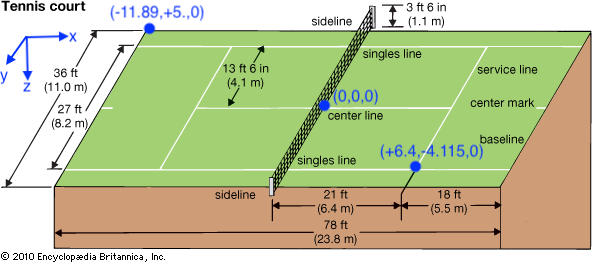
\includegraphics[width=1\linewidth]{image/tennis_court} \caption{Tennis Court}\label{fig:court}
\end{figure}

\hypertarget{overview-the-dataset}{%
\section{Overview the dataset}\label{overview-the-dataset}}

The data set Figure\ref{fig:datset} includes return impact for returned points in ATP singles matches for events between 2018 and 2020. There are 25 variables and 126455 observations in this data set and each observation refers to a single point within a match. From Figure\ref{fig:tidymiss}, there is no missing value in the data set, so we omit the data wrragling this step and use the data directly.

\begin{figure}
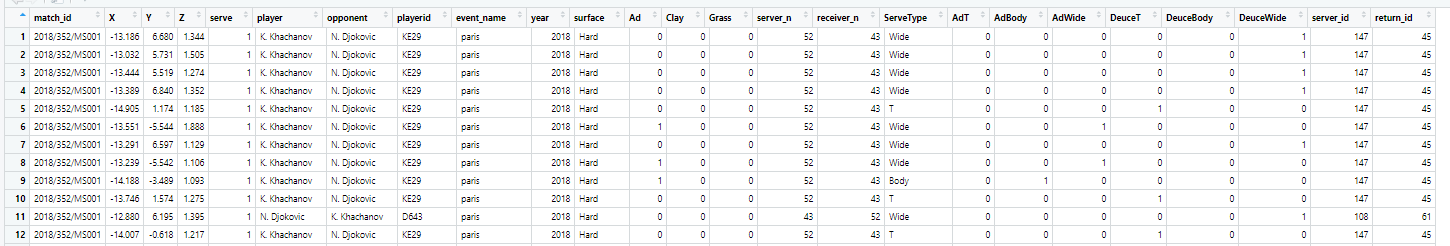
\includegraphics[width=1\linewidth]{image/dataset} \caption{Data set overview}\label{fig:datset}
\end{figure}

\begin{verbatim}
##    match_id               X                 Y                    Z         
##  Length:126455      Min.   :-23.111   Min.   :-10.587000   Min.   :-0.004  
##  Class :character   1st Qu.:-13.902   1st Qu.: -3.951000   1st Qu.: 1.191  
##  Mode  :character   Median :-12.841   Median :  0.782000   Median : 1.328  
##                     Mean   :-13.012   Mean   :  0.006236   Mean   : 1.344  
##                     3rd Qu.:-11.867   3rd Qu.:  2.903000   3rd Qu.: 1.493  
##                     Max.   : -6.423   Max.   : 10.212000   Max.   : 3.902  
##      serve          player            opponent           playerid        
##  Min.   :1.000   Length:126455      Length:126455      Length:126455     
##  1st Qu.:1.000   Class :character   Class :character   Class :character  
##  Median :1.000   Mode  :character   Mode  :character   Mode  :character  
##  Mean   :1.408                                                           
##  3rd Qu.:2.000                                                           
##  Max.   :2.000                                                           
##   event_name             year        surface                Ad        
##  Length:126455      Min.   :2018   Length:126455      Min.   :0.0000  
##  Class :character   1st Qu.:2019   Class :character   1st Qu.:0.0000  
##  Mode  :character   Median :2019   Mode  :character   Median :0.0000  
##                     Mean   :2019                      Mean   :0.4229  
##                     3rd Qu.:2020                      3rd Qu.:1.0000  
##                     Max.   :2020                      Max.   :1.0000  
##       Clay            Grass            server_n       receiver_n   
##  Min.   :0.0000   Min.   :0.00000   Min.   : 1.00   Min.   :10.00  
##  1st Qu.:0.0000   1st Qu.:0.00000   1st Qu.:16.00   1st Qu.:21.00  
##  Median :0.0000   Median :0.00000   Median :29.00   Median :32.00  
##  Mean   :0.1465   Mean   :0.05388   Mean   :28.18   Mean   :32.78  
##  3rd Qu.:0.0000   3rd Qu.:0.00000   3rd Qu.:37.00   3rd Qu.:38.00  
##  Max.   :1.0000   Max.   :1.00000   Max.   :66.00   Max.   :66.00  
##   ServeType              AdT             AdBody          AdWide      
##  Length:126455      Min.   :0.0000   Min.   :0.000   Min.   :0.0000  
##  Class :character   1st Qu.:0.0000   1st Qu.:0.000   1st Qu.:0.0000  
##  Mode  :character   Median :0.0000   Median :0.000   Median :0.0000  
##                     Mean   :0.1102   Mean   :0.138   Mean   :0.1747  
##                     3rd Qu.:0.0000   3rd Qu.:0.000   3rd Qu.:0.0000  
##                     Max.   :1.0000   Max.   :1.000   Max.   :1.0000  
##      DeuceT         DeuceBody         DeuceWide        server_id     
##  Min.   :0.0000   Min.   :0.00000   Min.   :0.0000   Min.   :  1.00  
##  1st Qu.:0.0000   1st Qu.:0.00000   1st Qu.:0.0000   1st Qu.: 50.00  
##  Median :0.0000   Median :0.00000   Median :0.0000   Median : 98.00  
##  Mean   :0.3154   Mean   :0.09277   Mean   :0.1689   Mean   : 99.94  
##  3rd Qu.:1.0000   3rd Qu.:0.00000   3rd Qu.:0.0000   3rd Qu.:151.00  
##  Max.   :1.0000   Max.   :1.00000   Max.   :1.0000   Max.   :205.00  
##    return_id    
##  Min.   : 1.00  
##  1st Qu.:21.00  
##  Median :39.00  
##  Mean   :41.05  
##  3rd Qu.:63.00  
##  Max.   :84.00
\end{verbatim}

\begin{figure}
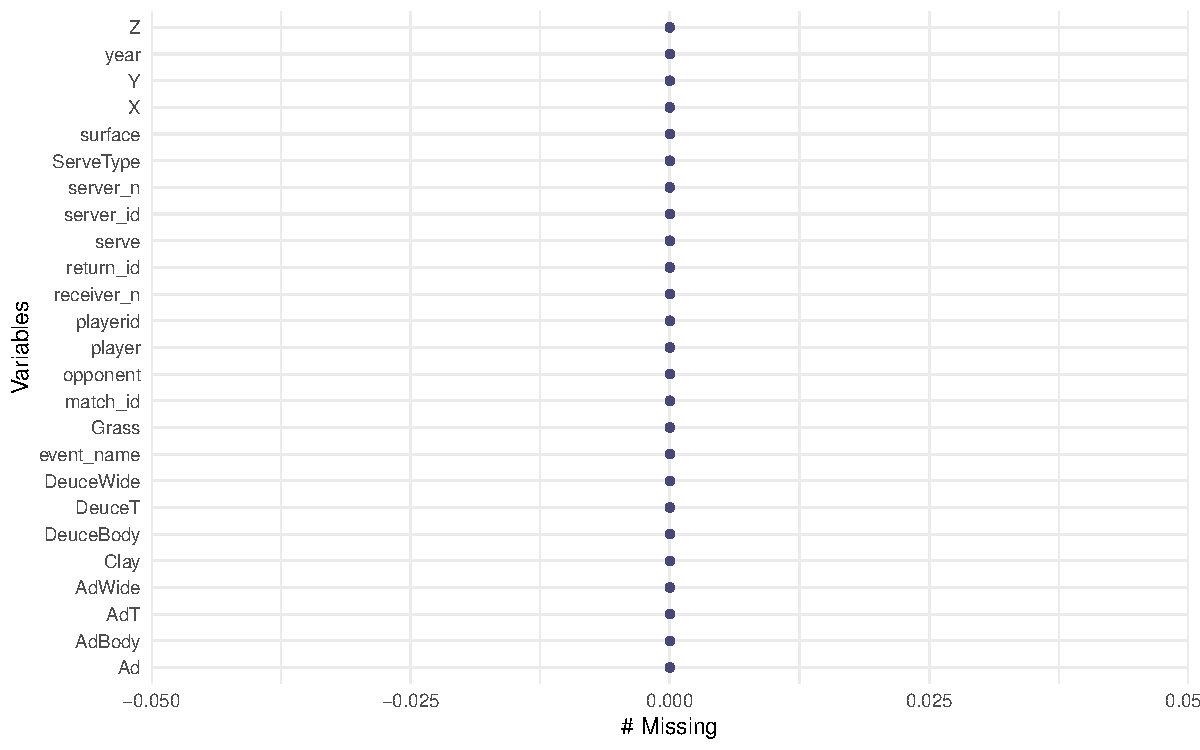
\includegraphics[width=1\linewidth]{Report_files/figure-latex/tidymiss-1} \caption{Check missing value}\label{fig:tidymiss}
\end{figure}

\hypertarget{how-variables-influence-players-return-impactimplementation}{%
\section{How variables influence player's return impact(Implementation)}\label{how-variables-influence-players-return-impactimplementation}}

\hypertarget{model-selection}{%
\subsection{Model selection}\label{model-selection}}

Started from the basic models to find out the relationship of the return impact.
* Logistic Regression

\begin{itemize}
\item
  Decision Tree
\item
  Random Forests
\item
  Gradient Boosting
\item
  Gaussian Mixture Model
\end{itemize}

\hypertarget{cluster-selection}{%
\subsection{Cluster Selection}\label{cluster-selection}}

The number of cluster components chose for the analysis was using the \texttt{Mclust} package that calculate their BIC and Figure \ref{fig:seronems} show the trend of the BIC.

\hypertarget{serve-one}{%
\subsection{serve one}\label{serve-one}}

\begin{verbatim}
## ---------------------------------------------------- 
## Gaussian finite mixture model fitted by EM algorithm 
## ---------------------------------------------------- 
## 
## Mclust EII (spherical, equal volume) model with 12 components: 
## 
##  log-likelihood     n  df       BIC       ICL
##        -8154922 74883 312 -16313347 -16315565
## 
## Clustering table:
##     1     2     3     4     5     6     7     8     9    10    11    12 
##  4949  4781  5238 12176  7012  4843  6042  6785  7124  5452  5233  5248
\end{verbatim}

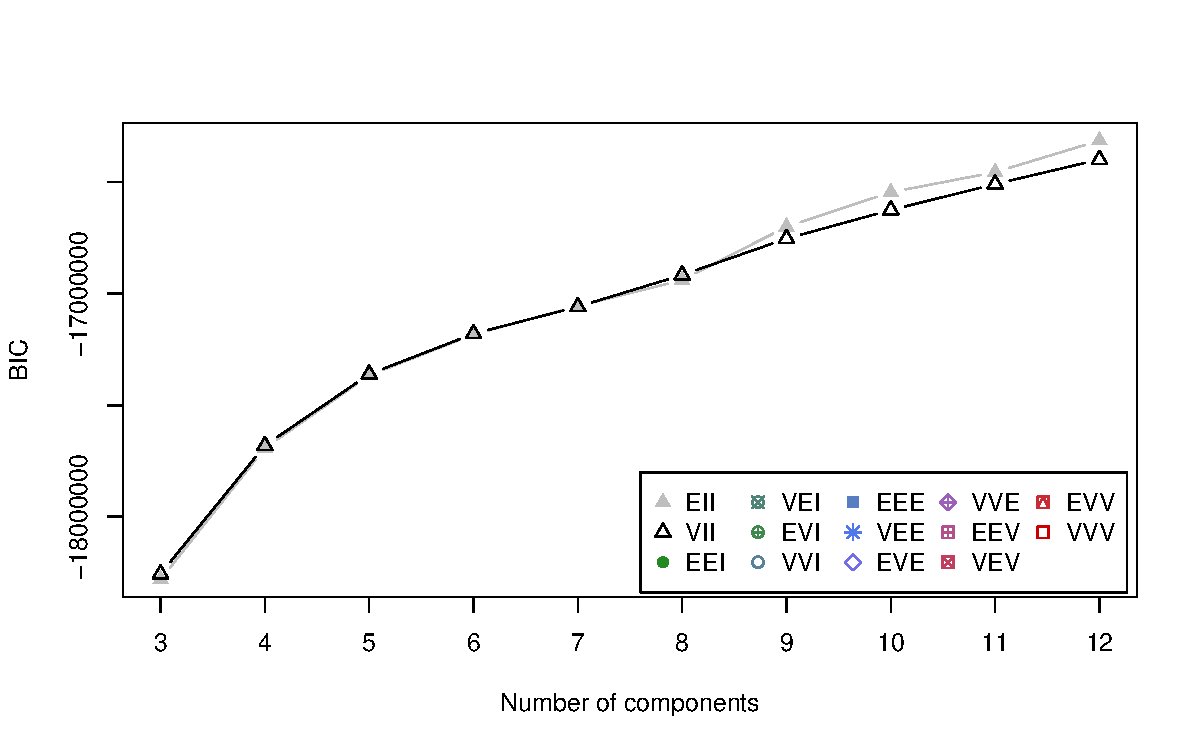
\includegraphics{Report_files/figure-latex/seronems-1.pdf}

\hypertarget{serve-two}{%
\subsection{serve two}\label{serve-two}}

\begin{verbatim}
## ---------------------------------------------------- 
## Gaussian finite mixture model fitted by EM algorithm 
## ---------------------------------------------------- 
## 
## Mclust VII (spherical, varying volume) model with 12 components: 
## 
##  log-likelihood     n  df       BIC       ICL
##        -5616451 51572 323 -11236406 -11237669
## 
## Clustering table:
##    1    2    3    4    5    6    7    8    9   10   11   12 
## 3995 3702 5181 3580 5262 3816 3000 3246 3564 8060 4199 3967
\end{verbatim}

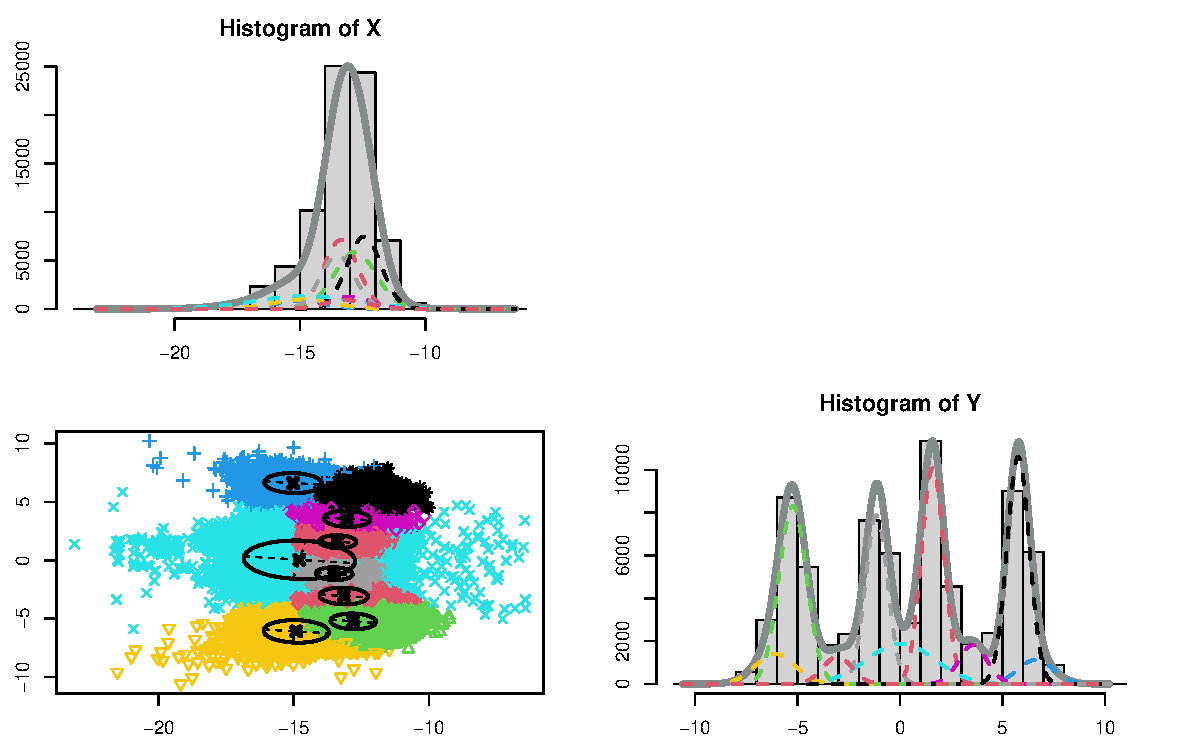
\includegraphics{Report_files/figure-latex/unnamed-chunk-3-1.pdf}

Compare to two serve of the difference number of cluster components' BIC, the number of 9 cluster perform well in the model. Thus, it will use 9 cluster for the rest analysis. In the shiny dashboard, there is a panel can run the function below to check the change of difference components cluster by selecting serve number, serve type, player, surface type.

\begin{verbatim}
## ****************************************
## *** INPUT:
## ****************************************
## * nbCluster =  9 
## * criterion =  BIC 
## ****************************************
## *** MIXMOD Models:
## * list =  Gaussian_pk_Lk_C 
## * This list includes only models with free proportions.
## ****************************************
## * data (limited to a 10x10 matrix) =
##       X      Y     
##  [1,] -13.19 6.68  
##  [2,] -13.03 5.731 
##  [3,] -13.44 5.519 
##  [4,] -13.39 6.84  
##  [5,] -14.9  1.174 
##  [6,] -13.55 -5.544
##  [7,] -13.29 6.597 
##  [8,] -13.24 -5.542
##  [9,] -14.19 -3.489
## [10,] -13.75 1.574 
## * ... ...
## ****************************************
## *** MIXMOD Strategy:
## * algorithm            =  EM 
## * number of tries      =  1 
## * number of iterations =  200 
## * epsilon              =  0.001 
## *** Initialization strategy:
## * algorithm            =  smallEM 
## * number of tries      =  10 
## * number of iterations =  5 
## * epsilon              =  0.001 
## * seed                 =  NULL 
## ****************************************
## 
## 
## ****************************************
## *** BEST MODEL OUTPUT:
## *** According to the BIC criterion
## ****************************************
## * nbCluster   =  9 
## * model name  =  Gaussian_pk_Lk_C 
## * criterion   =  BIC(594167.0499)
## * likelihood  =  -296875.8868 
## ****************************************
## *** Cluster 1 
## * proportion =  0.1911 
## * means      =  -13.3630 1.5874 
## * variances  = |     0.4737    -0.0298 |
##                |    -0.0298     0.2946 |
## *** Cluster 2 
## * proportion =  0.0429 
## * means      =  -14.9798 -6.1702 
## * variances  = |     1.4187    -0.0893 |
##                |    -0.0893     0.8824 |
## *** Cluster 3 
## * proportion =  0.2035 
## * means      =  -12.8196 -5.1903 
## * variances  = |     0.7719    -0.0486 |
##                |    -0.0486     0.4802 |
## *** Cluster 4 
## * proportion =  0.0323 
## * means      =  -15.0320 6.6422 
## * variances  = |     1.1014    -0.0693 |
##                |    -0.0693     0.6851 |
## *** Cluster 5 
## * proportion =  0.2019 
## * means      =  -12.4514 5.7605 
## * variances  = |     0.4761    -0.0300 |
##                |    -0.0300     0.2962 |
## *** Cluster 6 
## * proportion =  0.0387 
## * means      =  -12.9781 3.5837 
## * variances  = |     0.6530    -0.0411 |
##                |    -0.0411     0.4062 |
## *** Cluster 7 
## * proportion =  0.0708 
## * means      =  -14.7497 1.2513 
## * variances  = |     3.8013    -0.2393 |
##                |    -0.2393     2.3645 |
## *** Cluster 8 
## * proportion =  0.0964 
## * means      =  -14.0630 -1.8374 
## * variances  = |     2.0216    -0.1272 |
##                |    -0.1272     1.2575 |
## *** Cluster 9 
## * proportion =  0.1223 
## * means      =  -13.4413 -1.0902 
## * variances  = |     0.3865    -0.0243 |
##                |    -0.0243     0.2404 |
## ****************************************
\end{verbatim}

\begin{verbatim}
## [1] 1
\end{verbatim}

\begin{verbatim}
## [1] 2
\end{verbatim}

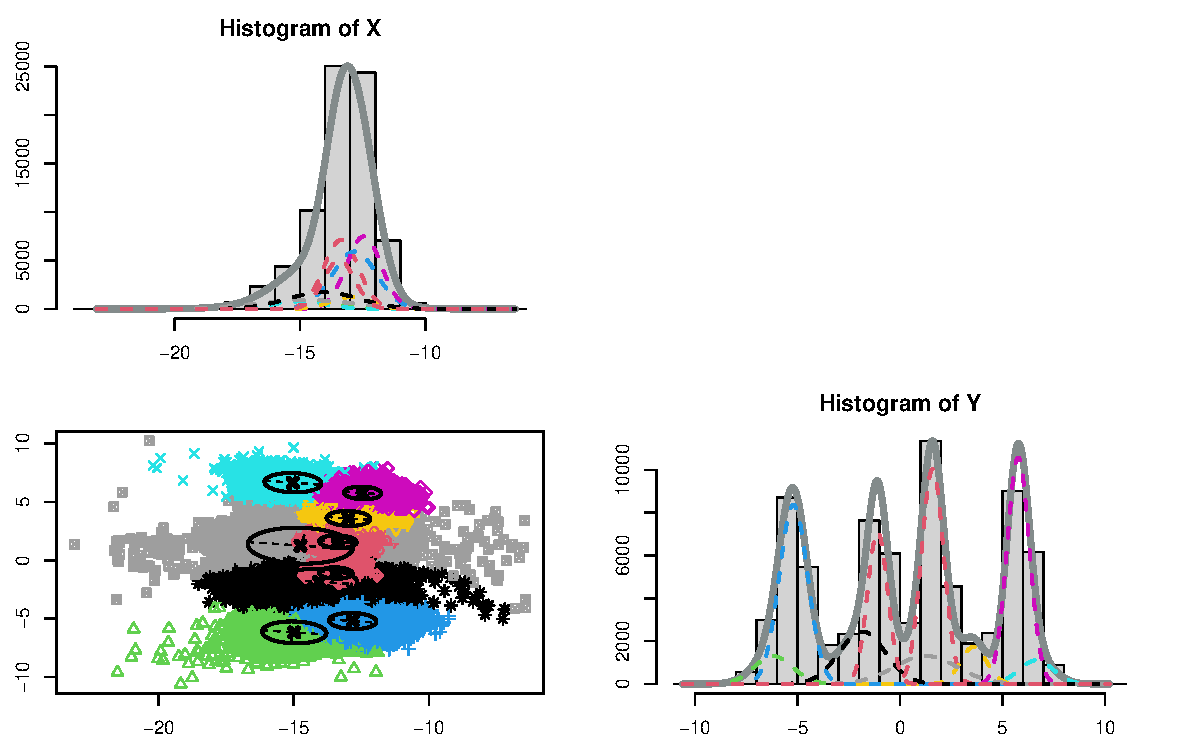
\includegraphics{Report_files/figure-latex/unnamed-chunk-4-1.pdf}

Under the result used the GMM model, there is a further discussion of the return impact base on the player, the match intensity increase and the rest of the variables.

\hypertarget{the-strategy-of-top-3-players-return-impact-positions}{%
\subsection{The strategy of top 3 players' return impact positions}\label{the-strategy-of-top-3-players-return-impact-positions}}

Are the top players have large difference of the return impact positions? Or similar.

\hypertarget{any-ajust-strategy-in-the-promotion-event-especially-the-final-round}{%
\subsection{Any ajust strategy in the Promotion event especially the final round?}\label{any-ajust-strategy-in-the-promotion-event-especially-the-final-round}}

Will player stand near or far away from the court during the semi-final ground? Or final ground?

\hypertarget{how-are-surface-type-influence-playersperformance}{%
\subsection{How are surface type influence players'performance?}\label{how-are-surface-type-influence-playersperformance}}

As grass and clay surface type have some slightly difference and will they influence the return impact positions?

\hypertarget{atp-lefties-in-the-top-100-rankings-return-impact}{%
\subsection{ATP Lefties In The Top 100 Rankings' return impact}\label{atp-lefties-in-the-top-100-rankings-return-impact}}

Are the player will have similar return impact positions because they are left hand users?

\hypertarget{will-they-change-stategy-when-were-facing-familar-player}{%
\subsection{(will they change stategy when were facing familar player)}\label{will-they-change-stategy-when-were-facing-familar-player}}

Compare head-to-head history result, find out the player have larger win proportion and compare their each game return impact positions.

\hypertarget{dashboard-user-guide}{%
\section{Dashboard User Guide}\label{dashboard-user-guide}}

\hypertarget{conclusion}{%
\section{Conclusion}\label{conclusion}}

\printbibliography[title=Reference]

\end{document}

